%!TEX root = paper.tex
%%%%%%%%%%%%%%%%%%%%%%%%%%%%%%%%%%%%%%%%%%%%%%%%%%%%%%%%%%%%%%%%%%%%%%%%%%%%%%%%
\section{Simulation Model}
\label{sec:simulation}

Based on the model introduced in Section~\ref{sec:model} a stochastic \gls{DES} was created that implements this model. This R-based simulator strifes to translate all of the earlier discussed lag blocks, while keeping them as configurable as possible.

By using a vector-based statistics language the core loop is kept compact and easy to modify and reorder to adapt to new scenarios in addition to the ones evaluated here. Due to the influence of several stochastic processes and the differing offset of the clocked processes, a sufficient number of repetitions is required to provide meaningful results. This is achieved by running large numbers of simulations in parallel through the built-in R facilities.

This section presents simulation results on each of the flavors of how to play video games: the local, online, and the cloud scenario.

The investigations here are not intended to cover every aspect of all parameters or to conduct full parameter studies, but are rather intended to highlight some particular aspect in each of the scenario. 

All of the source code and the data from the upcoming scenarios is provided in the simulation-folder\footnote{\url{https://github.com/mas-ude/onlinegame-lag-sim/tree/master/simulation}} of the repository and can be used as public domain.


\subsection{Parameters}

Besides being fully reconfigurable, the simulation currently also has a few default parameters set and makes assumptions that go beyond what the base end-to-end model implies for reasons of simplicity.
First, the input is modeled by an exponential distribution with a rate of $20$ events per second. \textbf{TODO:} implications and reasons?

Additionally, the rate at which command messages are sent to the game server is set equal to the server's tickrate as the server would not process more commands either way. This might however increase the end-to-end lag in some situations if a command message just misses one of the server's ticks and has to wait another full cycle.


%%%%%%%%%%%%%%%%%%%%%%%%%%%%%%%%%%%%%%%%%%%%%%%%%%%%%%%%%%%%%%%%%%%%%%%%%%%%%%%%
\subsection{Local Games}

The first and simplest scenario to be investigated here, is the case of the local game. In the version implemented here, the tickrate is still present, but the influence of the network is entirely removed. It therefore represents the best-case an online multiplayer game could achieve, when the server would run locally.

\begin{figure}[!t]
	\centering
	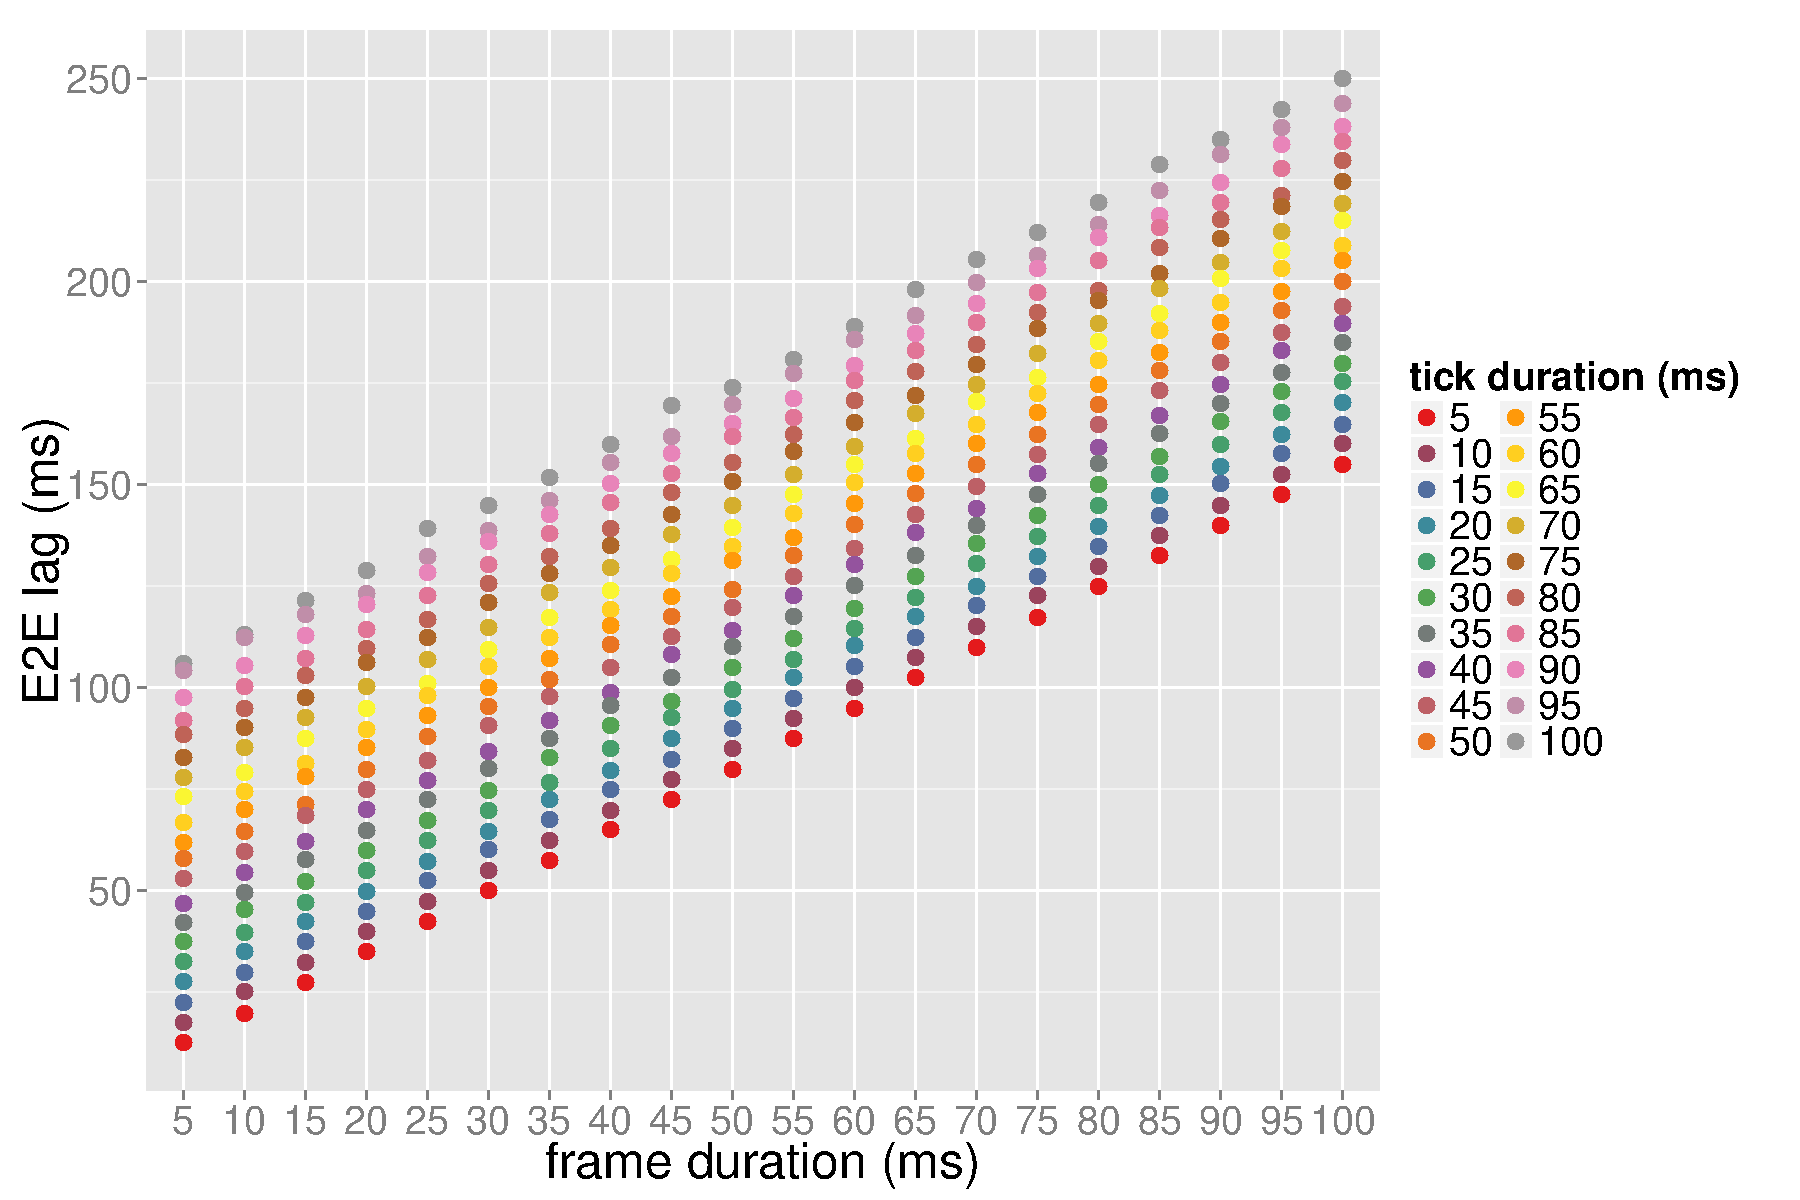
\includegraphics[width=1.0\columnwidth]{../simulation/visualization/nwless-onlinegame-1000rounds.pdf}
	\caption{Scatterplot of the median E2E lag under various frame and tick durations in a scenario where the game is running fully local.}
\label{fig:nwless-scatter}
\end{figure}

Figure~\ref{fig:nwless-scatter} presents a scatter plot of the relationship between the frame duration (i.e., the inverse of the framerate), the tick duration, and the resulting end-to-end lag.



%%%%%%%%%%%%%%%%%%%%%%%%%%%%%%%%%%%%%%%%%%%%%%%%%%%%%%%%%%%%%%%%%%%%%%%%%%%%%%%%
\subsection{Online Gaming}

\begin{figure}[!t]
	\centering
	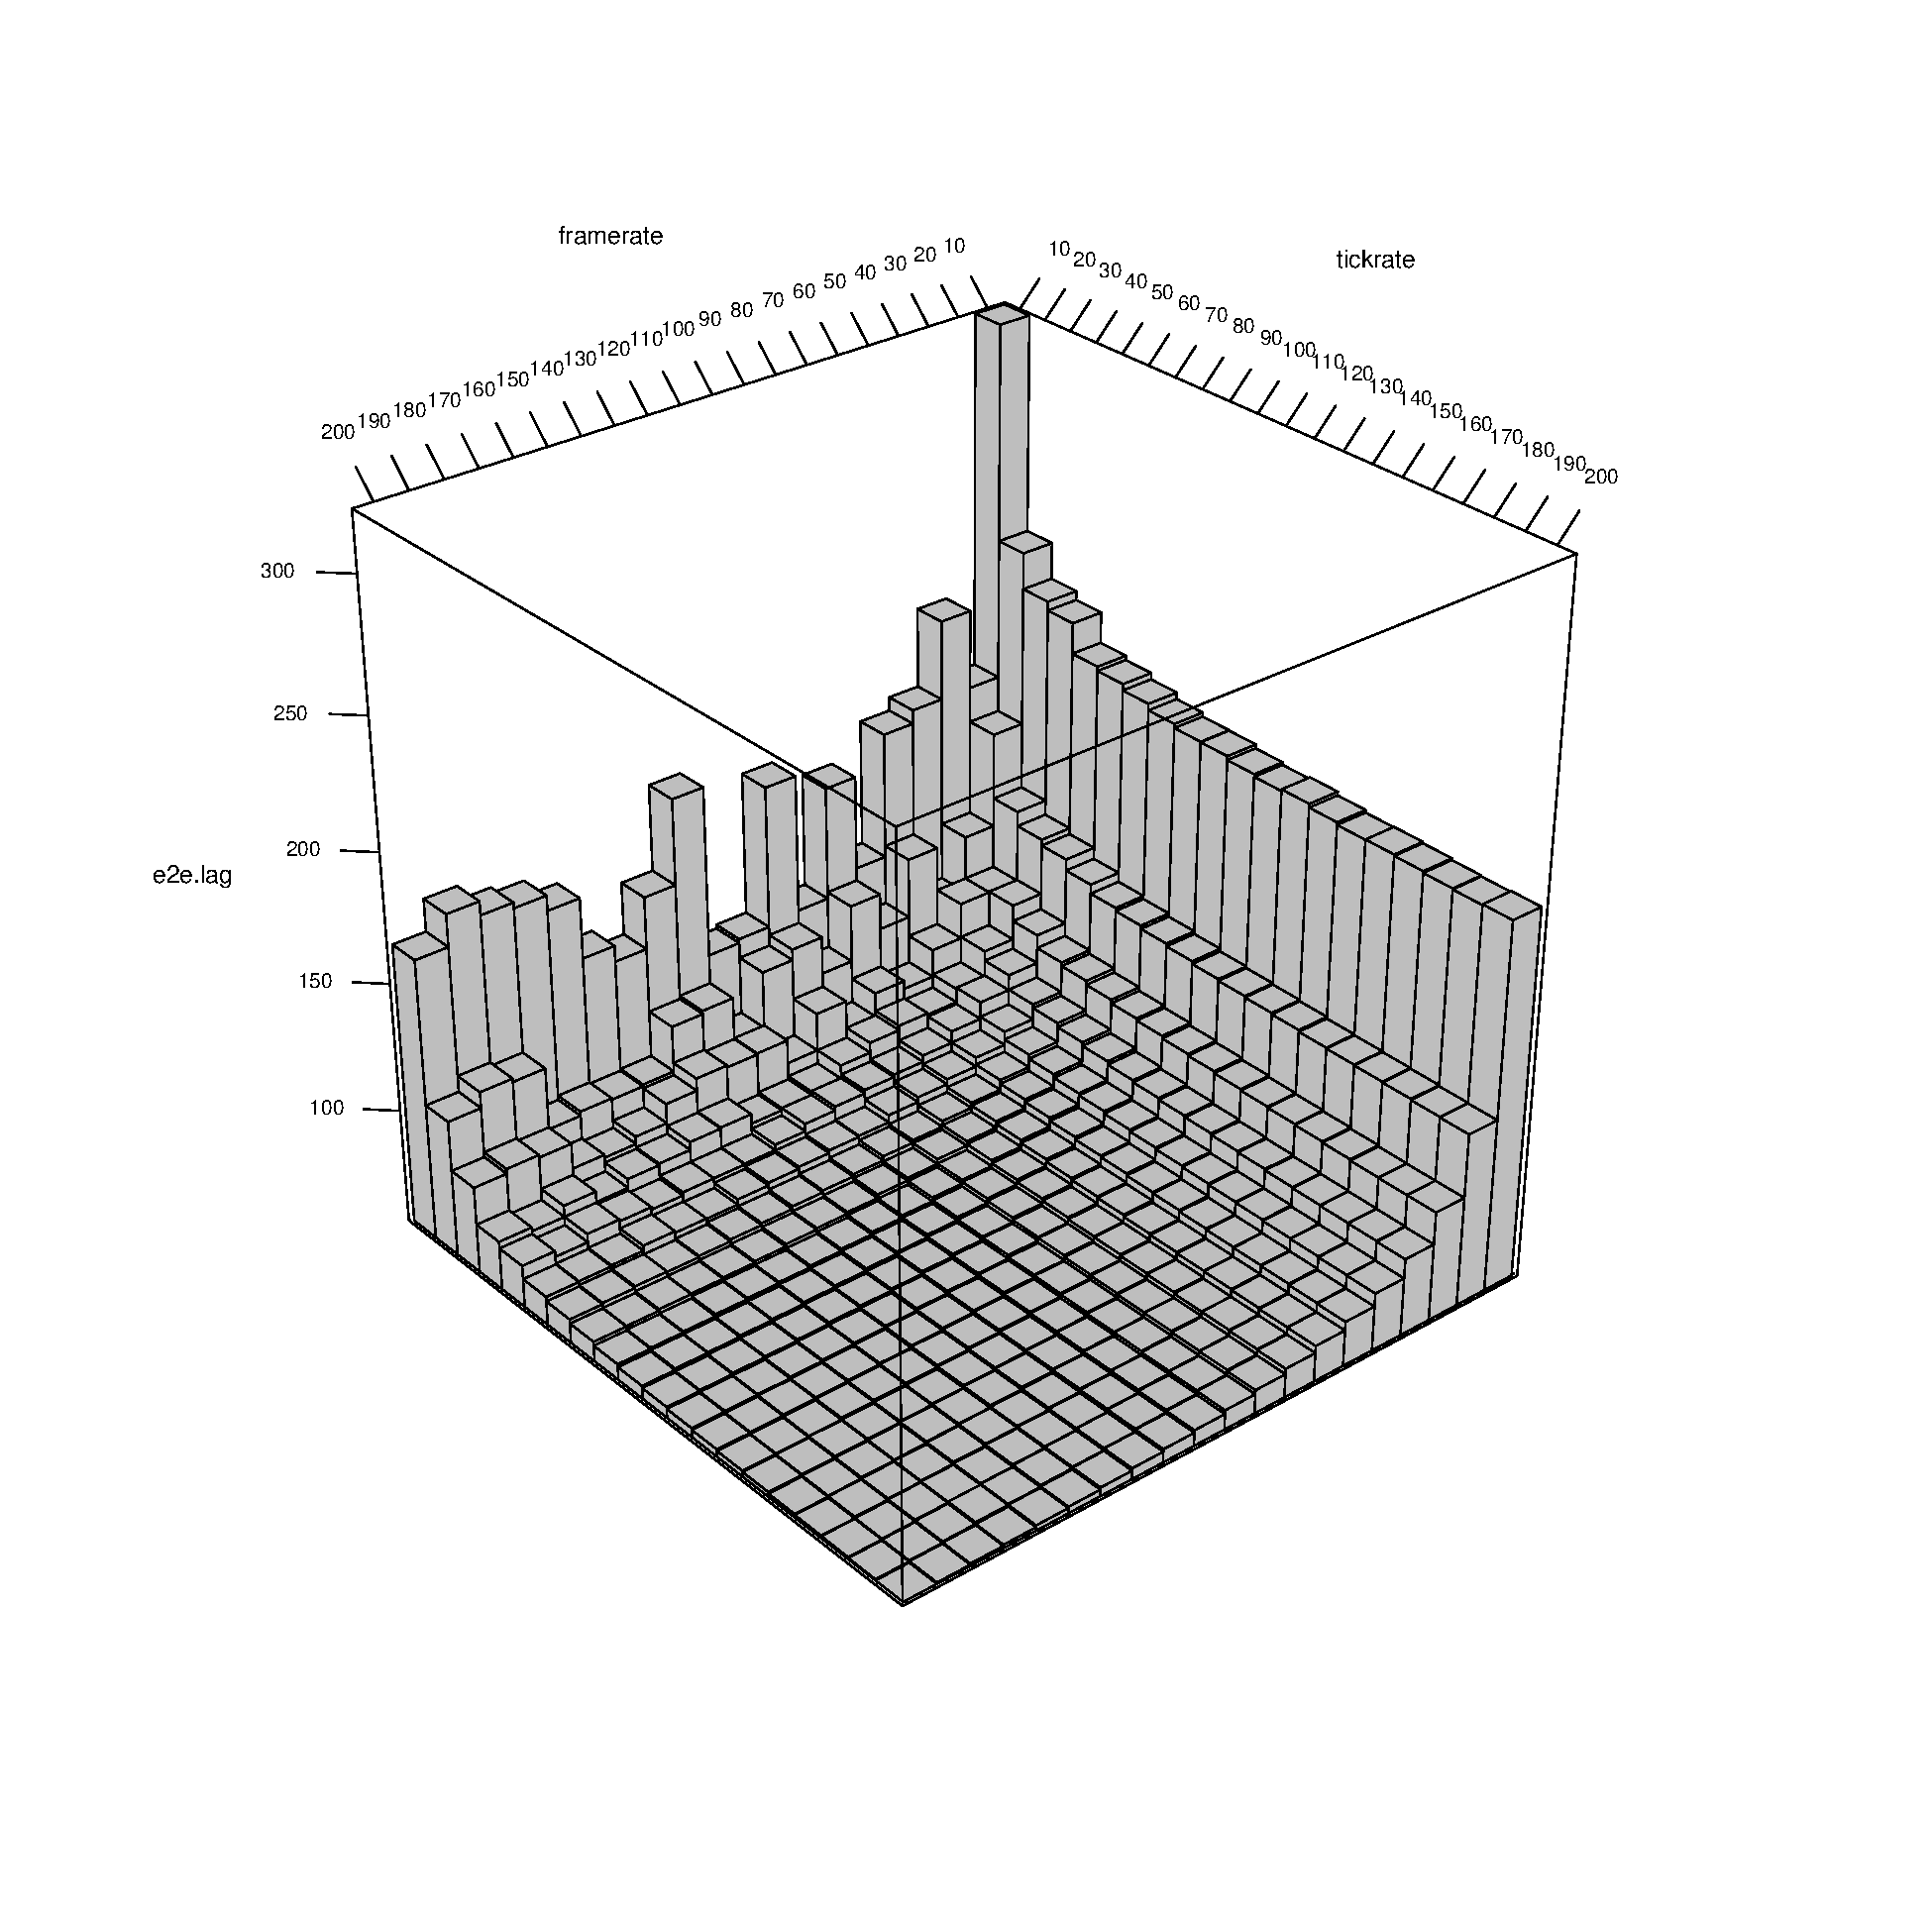
\includegraphics[width=1.0\columnwidth]{../simulation/visualization/e2e-lag-3dbars.pdf}
	\caption{3D bars representation of the influence of both the client's framerate and the server's tickrate on the end-to-end lag in the online game scenario.}
\label{fig:3dbars-framerate-tickrate-lag}
\end{figure}

Figure~\ref{fig:3dbars-framerate-tickrate-lag} ...

To note here: Variance on the framerate axis is much higher than for the tickrate. This has practical implications for gaming studies. Experiment that examine the influence of the framerate need to have a very high repetition rate to keep the variance low and provide meaningful results.


%%%%%%%%%%%%%%%%%%%%%%%%%%%%%%%%%%%%%%%%%%%%%%%%%%%%%%%%%%%%%%%%%%%%%%%%%%%%%%%%
\subsection{Cloud Gaming}


\begin{figure}[!t]
	\centering
	%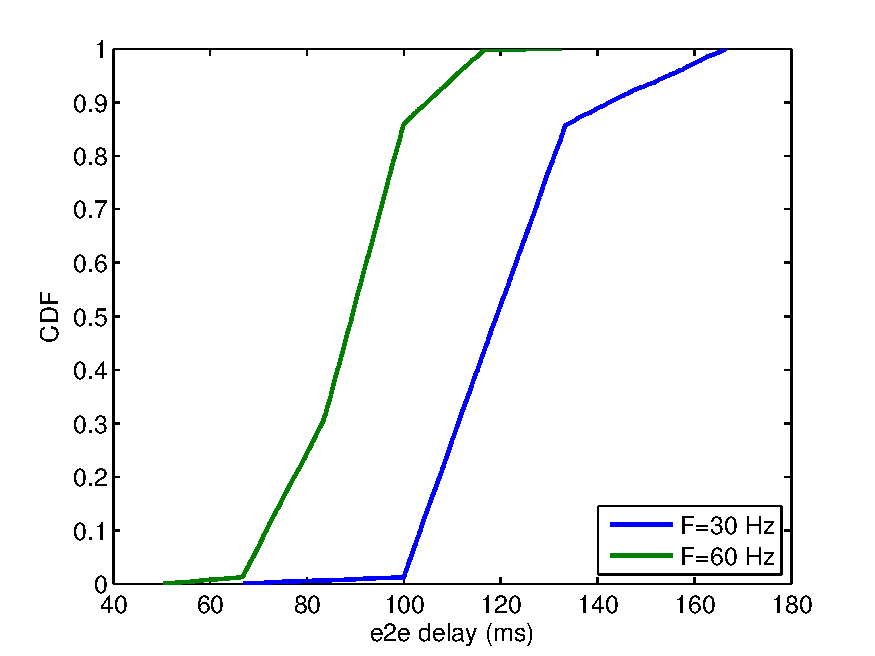
\includegraphics[width=1.0\columnwidth]{images/e2e-delay-sim.pdf}
	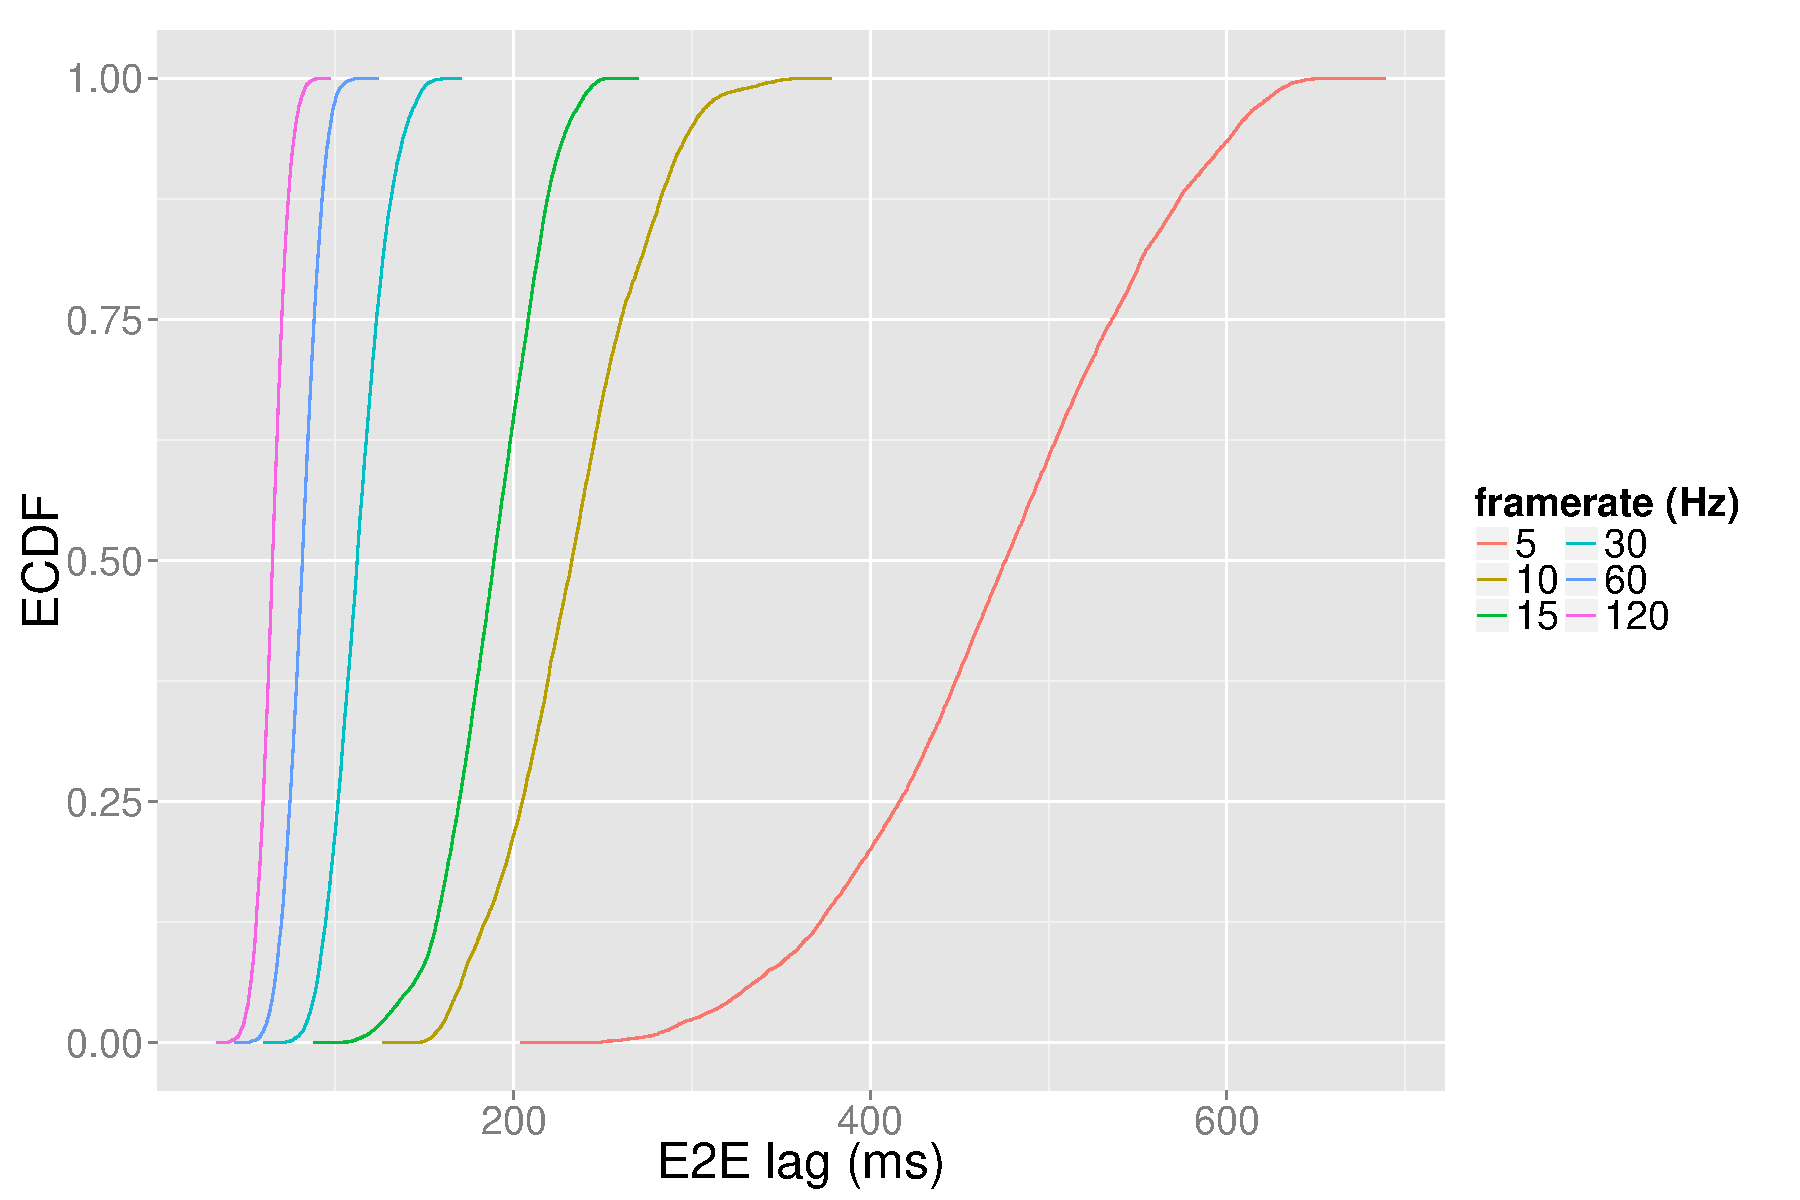
\includegraphics[width=1.0\columnwidth]{../simulation/visualization/cloudgaming-lag-cdf.pdf}
	\caption{\acrshort{ECDF} of the influence of the server's rendering and streaming framerate on the end-to-end lag in the cloud gaming scenario.}
\label{fig:cloud-e2e-delay-sim}
\end{figure}

Figure~\ref{fig:cloud-e2e-delay-sim}...


%%%%%%%%%%%%%%%%%%%%%%%%%%%%%%%%%%%%%%%%%%%%%%%%%%%%%%%%%%%%%%%%%%%%%%%%%%%%%%%%
\subsection{Discussion}



% Ultimately, to capture any and all latency sources in gaming you would need to rely on external recording gear.
% With modified input: zero latency and visible input detection (e.g. solder some LEDs to the buttons)

% Also Arduino with photodiode method described in \cite{beyermethod}
% Both this and camera method also work for closed game consoles


%%%%%%%%%%%%%%%%%%%%%%%%%%%%%%%%%%%%%%%%%%%%%%%%%%%%%%%%%%%%%%%%%%%%%%%%%%%%%%%%
%\subsection{Evaluated Metrics}

%%%%
%\subsubsection{Frame Rates and Frame Times (i.e. frame IAT)}
%i.e. frame IAT
%Reasoning for frame IAT and the negligence of past investigations
%%%%
%\subsubsection{Total and additional end-to-end latency}
%physical controller input to in-game reaction
%different in-game actions have already difference in latency, therefore need to test various actions for a complete picture
%Also discuss RTT as Hz (1/RTT) as measure for interactivity


%%%%%%%%%%%%%%%%%%%%%%%%%%%%%%%%%%%%%%%%%%%%%%%%%%%%%%%%%%%%%%%%%%%%%%%%%%%%%%%%
%\subsection{Reasonable Configuration/Setting Ranges to Test}

% Resolution: Minimum 720p, 1080p recommended, even higher is better (1440p or 2160p)
% Frame rate: 60 fps very much recommended, 30 absolute minimum,  120 or 144 can also be feasible
% Configure games to run at high or at least medium settings
% For console games: use the games intended settings for the console, never downscale the game or reduce the frame rate for streaming
% Assume no network latency higher than 200ms, preferably less than 100ms
% Assume typical access link conditions, i.e. no less than 10-16Mb/s



%Works only for general purpose computing devices with full access.
%Easiest method, but might not capture full end-to-end latency.
%FRAPS, OBS, DirectX Hooking, MSI Afterburner
%FCAT as hybrid solution with external capture card and computer


% \url{http://www.red.com/learn/red-101/high-frame-rate-video}


% articles:
% why frametimes
%     \url{https://techreport.com/review/21516/inside-the-second-a-new-look-at-game-benchmarking}

% Inside the second with Nvidia's frame capture tools
%     \url{https://techreport.com/review/24553/inside-the-second-with-nvidia-frame-capture-tools}

 % As the second turns: the web digests our game testing methods
 %    \url{https://techreport.com/blog/24133/as-the-second-turns-the-web-digests-our-game-testing-methods}

% GPU Reviews: Why Frame Time Analysis is important
%     \url{http://www.vortez.net/articles_pages/frame_time_analysis.html}

% Durante's Witcher 3 analysis: the alchemy of smoothness
%     \url{http://www.pcgamer.com//durantes-witcher-3-analysis-the-alchemy-of-smoothness/}


% Analysing Stutter – Mining More from Percentiles
%     \url{https://developer.nvidia.com/content/analysing-stutter-%E2%80%93-mining-more-percentiles-0}

% fraps vs fcat method
%     \url{http://www.extremetech.com/gaming/154089-after-almost-20-years-gpu-benchmarking-is-moving-past-frames-per-second}

% FRAPS + FRAFS
% \url{http://www.fraps.com/}
% \url{http://sourceforge.net/projects/frafsbenchview/}
% \url{http://www.5group.com/wordpress/2012/07/14/gpu-mist-pre-release-1-0-rc1/}

% issue: Fraps measures the flip queue input rather then the actual render output frames which is fine when measuring FPS but is rather poor if you want to measures actual frame times and analyze microstutter.


% NVIDIA FCAT
% \url{http://www.geforce.com/hardware/technology/fcat}
% \url{http://www.overclockers.com/nvidias-fcat-gpu-testing-pursuing/}


% Valve for Linux GL Games
% \url{https://github.com/ValveSoftware/voglperf}

% Info über MSI Afterburner overlay? oder GF experience? GPU-Z? Rivatuner Statistics Server?
% \url{http://www.overclock.net/a/how-to-use-rivatuner-afterburner-on-screen-display-and-more}



% \url{https://en.wikipedia.org/wiki/Game_classification}
% \url{https://en.wikipedia.org/wiki/Video_game_genre}
% \url{https://en.wikipedia.org/wiki/List_of_video_game_genres}

